

\emph{Automated deduction}, also called \emph{automated theorem proving} or simply
\emph{theorem proving}, is the study of
automatically constructing formal proofs in symbolic logics.  A \emph{theorem prover}
is a software system that attempts to construct such proofs.  In first-order
classical logic, much progress has been made in the design and implementation
of algorithms for
efficient deduction.  Vampire~\cite{Voronkov.1999.CADE} is used in
Microsoft's Spec\# software verification tool.
EQP famously resolved the Robbins Conjecture, an open question
in boolean algebra.  Waldmeister, a first-order prover for equational
logic, is incorporated into Mathematica.

Progress in theorem proving in non-classical logics has been less pronounced.
A fundamental difficulty is that mature theorem provers tend to be large programs.
As of the time of writing, Vampire has 160k lines of code, while
Prover9, the successor to EQP, has 112k.  Because implementing theorem provers
is a difficult and time-consuming task, the complexity of implementation
is a disincentive for experimenting with
non-classical logics to model a new domain, even if that logic may be well-suited
for the task at hand.

Wallen, in his 1990 thesis on automated-deduction in non-classical logic, writes

\vspace{1em}

\noindent
\textit{The aim has been to lay the groundwork for a theory of automated deduction in
arbitrary symbolic logics by providing empirical evidence for the existence of
a \emph{uniform} approach to efficient proof search in both truth-functional and
non truth-functional logics.  Whilst the formulation of such a comprehensive
theory is at the time of writing beyond the author's reach, it is intended that
the form such a theory might take, and the ideas on which it might be based, be
suggested by the methods brought to bear in the text.}~\cite{Wallen.1990.Book}

\vspace{1em}


From a practical point of view, one may reasonably ask,
what use is non-classical logic?  intuitionistic logic

In~\citep{Gurevich.2009.DKAL2}, Gurevich writes,
while experimenting with logics in which to express authentication protocols,

\noindent
\begin{quote}
Eventually we switched from algebra to logic that treats $x ^ y$ and $x~!~y$ as
conjunction and implication respectively. And something unexpected happened,
a little miracle. The logic of infons happened to be a natural and conservative
extension of disjunction-free intuitionistic logic.
\end{quote}


This thesis continues Wallen's efforts toward uniform methods for
efficient proof search in symbolic logics.  While Wallen's framework
was founded on a matrix approach, we use a dual approach based on the
inverse method.  Like resolution in classical
logic, the inverse method is a bottom-up, saturation-based proof procedure.
Unlike resolution, which relies on strong clause normal forms for its
effectiveness, the inverse method is based on the sequent calculus.
Thus, it can be used with logics where no clausal normal forms exist such as
intuitionistic logic.


\paragraph{Intuitionistic logic.}

Intuitionistic logic arose during the foundational tumult of the early 20th
century.  The schism between classical and intuitionistic logic
is essentially captured by Brouwer's rejection of
the classical tautology $A \Or \Not A$ for any proposition $A$, also known as
the \emph{law of the excluded middle}.  The difficulty with the law is that it
may not be possible, even in principle\footnote{Though this was not formally
understood until G\"odel's first incompleteness theorem of 1931.}, to prove
either $A$ or $\Not A$ separately.  To get a sense of Brouwer's discomfort,
consider Fermat's Last Theorem (FLT):

\[
\All x\ y\ z\ n.\ n > 2 \Imp \Not (x^n + y^n = z^n)
\]

\newcommand{\FLT}{\mbox{FLT}}
\newcommand{\TPC}{\mbox{TPC}}

\noindent
Until 1995, it was unknown whether FLT was provably true, provably
false, or neither.  In this light, the tautological status of
$\FLT \Or \Not \FLT$ seems open to question.
Once Wiles' proof was published, one could with greater certainty assert
$\FLT \Or \Not \FLT$.   Still, it is always possible to select some other
open problem such as the twin primes conjecture (TPC), and the argument
above still holds.
Given the state of the world in 2012,
$\FLT \Or \Not \FLT$ is intuitionistically provable (with much hard work)
but $\TPC \Or \Not \TPC$ is not.
In classical logic, both are trivial tautologies.

The development of intuitionistic logic during the 20th century led to rich new
branches of mathematics, such as constructive analysis and intuitionistic
number theory.  Its
study also elucidated connections between intuitionistic logic and type systems
of functional programming languages via the Curry-Howard isomorphism, directly
influencing programming language design.  Systems such as
Martin-L\"of's intuitionistic type theory and the calculus of inductive constructions
provided an intuitionistic foundation for mathematics.

% What is theorem proving

Meanwhile, the development of modern computer hardware made the implementation
of proof search algorithms increasingly practical.  The field of
\emph{automated theorem proving} (or just \emph{theorem proving})
studies the design and implementation of algorithms that prove theorems in
formal systems (such as classical and intuitionistic logic) automatically.
Improvements in theorem proving for classical logic have been dramatic.
Probably the first theorem-proving algorithm that was implemented on a physical machine was
Martin Davis' 1954 implementation of Presburgher's algorithm for deciding linear
integer arithmetic, whose ``great triumph was to prove that the sum of two even numbers
is even''~\cite{Davis.2001.History}.  Only six decades later,
modern classical theorem provers
have evolved to the point that that have resolved open mathematical
problems such as the Robbins conjecture~\cite{McCune.JAR.1997}.

Applications of theorem proving to computer science abound.
Hardware verification uses classical propositional logic
to encode circuit design and uses SAT solvers to prove that the design
adequately represents the intended behavior of the circuit on all inputs.
Software verification is another example,
where tools such as Microsoft's \emph{Spec\#}~\cite{Barnett.2005.CASSIS} are able to
statically check verification conditions and loop invariants.  Spec\# uses
different kinds of classical theorem provers, such as
Vampire~\cite{Voronkov.1999.CADE} for general first-order theorem proving
and the SMT solver Z3~\cite{Moura.2008.TACAS} to solve arithmetic constraints.
In theorem proving for
hybrid systems, Platzer's KeYmaera
tool~\cite{Platzer.2008.IJCAR} uses classical theorem provers (such as Z3)
as subroutines to prove safety properties of systems such as the
European Train Control System~\cite{Platzer.2009.ICFEM}.

While automated deduction in
classical logic is a mature field, with dozens of theorem provers and an
annual competition, deduction in nonclassical logics has been
comparitively neglected\footnote{A notable exception is model checking in temporal
logic}.
Less attention has been paid to the theorem proving problem in intuitionistic
logics.  The primary reason for this is simply that classical logic is a far
more
common modeling language in computer science.  Moreover, even when an
intuitionistic model would be more precise or succinct than a classical model,
the complexity of theorem proving in intuitionistic logic can be a barrier.  It
is strictly more difficult than classical theorem proving; the propositional
fragment is PSPACE-complete while the classical analog is merely NP-complete,
while classical first-order logic can be embedded in intuitionistic logic.
Advances from the classical literature can not normally be used in
intuitionistic theorem
proving, as such advances requently rely on peculiarities of classical logic
itself.  For example, classical logic admits very simple quantifier-free normal
forms which do not exist in intuitionistic logic.

Existing proof search strategies for intuitionistic logic are
based on the \emph{sequent calculus}, a formalism due to Gentzen from 1934.
The primary problem with using the sequent calculus for proof search
is redundancy; there are generally many ways to prove the same theorem,
resulting in an unnecssarily large search space.
Andrioli's 1992 discovery of
\emph{focusing} showed that the search space of the sequent calculus can
be dramatically reduced by analyzing the \emph{polarities} of subformulas of
a goal formula.

Formerly, all intuitionistic theorem proving was
accomplished using tableaux or matrix-style searches in an unfocused
sequent calculus.

In this thesis we argue that focusing,
combined with a resolution-like procedure called the inverse-method,
is an efficient and flexible means to implement theorem provers for
intuitionistic logics.

\paragraph{Thesis}
The polarized inverse method provides an efficient and flexible means for proof
search in non-classical logics.

\bigskip

\noindent
Besides its theoretical interest, proof search in IL has some practical
applications.

\paragraph{Proof assistants}
Proof assistants are programs that assist a human mathematician
formally verify theorems from first principles.  Unlike in informal
mathematics, which elides the bulk of the underlying logical operations
involved, a proof assistant carries out reasining directly in the
underlying logic, making a record of proof steps.  Most proof assistants
attempt to automate tedious logical steps so the human can focus only
on the high-level details of the proof.  While this does not always
work in practice due to the limitations of automated reasoning, automated
reasoning is still a vitally important part of the day-to-day use of
proof assistants.  For example, in both the classical proof assistant
HOL-Light and the intuitionistic proof assistant Coq, the automated
strategies (``MESON'' and ``auto'' respectively) are used more than
any other operation but rewriting and basic hypothesis management
(with 13k and 10k calls respectively in the latest source code).

\paragraph{Authentication}
Intuitionistic authentication logics have been
developed~\cite{Garg.2010.SSP, Gurevich.2008.DKAL}
to reason about communication and file-access protocols.

\paragraph{The contributions of this thesis.}

This thesis describes a novel method of theorem proving in
the following intuitionistic logics:

\begin{itemize}
\item Propositional  (Chapter~\ref{chapter.prop})
\item First-order (Chapter~\ref{chapter.fol})
\item Modal logic in the style of Simpson (Chapter~\ref{chapter.modal})
\item Modal logic in the style of Pfenning-Davies (Chapter~\ref{chapter.pd})
\item Linear logic (Chapter~\ref{chapter.linear})
\item Ordered logic (Chapter~\ref{chapter.ordered})
\end{itemize}

\noindent
The basis of the theorem provers is a polarized, focused, first-order sequent
calculus with constraints, using the inverse method to exhaustively search for
proofs.  For each logic we prove soundness and completeness of the system, and
provide an implementation.  The implementation details form a significant
part of the contributions of this thesis, as considerable
optimizations, at all levels of abstraction, were
necessary to make the performance of the generic method acceptable.
In cases where other theorem provers exist, we
provide performance comparisons with the other techniques.  In propositional
logic, our method is competitive with the best existing systems.  Our
first-order prover surpasses existing systems.  Our linear prover, while
able to solve simple problems, is not competitive with the other prover for full
first-order linear logic, Chaudurhi's Linprover (though with some effort we
believe it can be made competitive).  Ours is the only theorem prover
for both flavors of modal logic, and ordered logic.


\section{Motivation}

\paragraph{Application: Proof-carrying authentication.}

\paragraph{Application: Type systems for distributed computing.}


\paragraph{Application: Program verification using proof assistants.}

In each of the above applications, the theorem proving problem is fundamental.
While theorem proving in classical logic has a vast body of literature and at
least a dozen mature implementations, less work has gone into the problem of
building practical theorem provers for non-classical logics.  This thesis
describes a flexible and efficient means of proof search called the
\emph{polarized inverse method}.  It is \emph{flexible} because it can be
applied to a variety of different logics, namely those satisfying the subformula
property and cut elimination.  It is \emph{efficient} due to a number of
optimizations to sequent calculi that greatly reduce the search space.

We give evidence for our thesis statement by describing and implementing the
polarized inverse method for a sequence of non-classical logics, shown in
Figure~\ref{graffle.logics}
and described
below.  In each case, our implementation is competitive with or superior to
existing theorem provers, or is the only known theorem prover for the logic.

\section{Contributions}

\section{Outline}
% 
\begin{figure}
  \begin{center}
    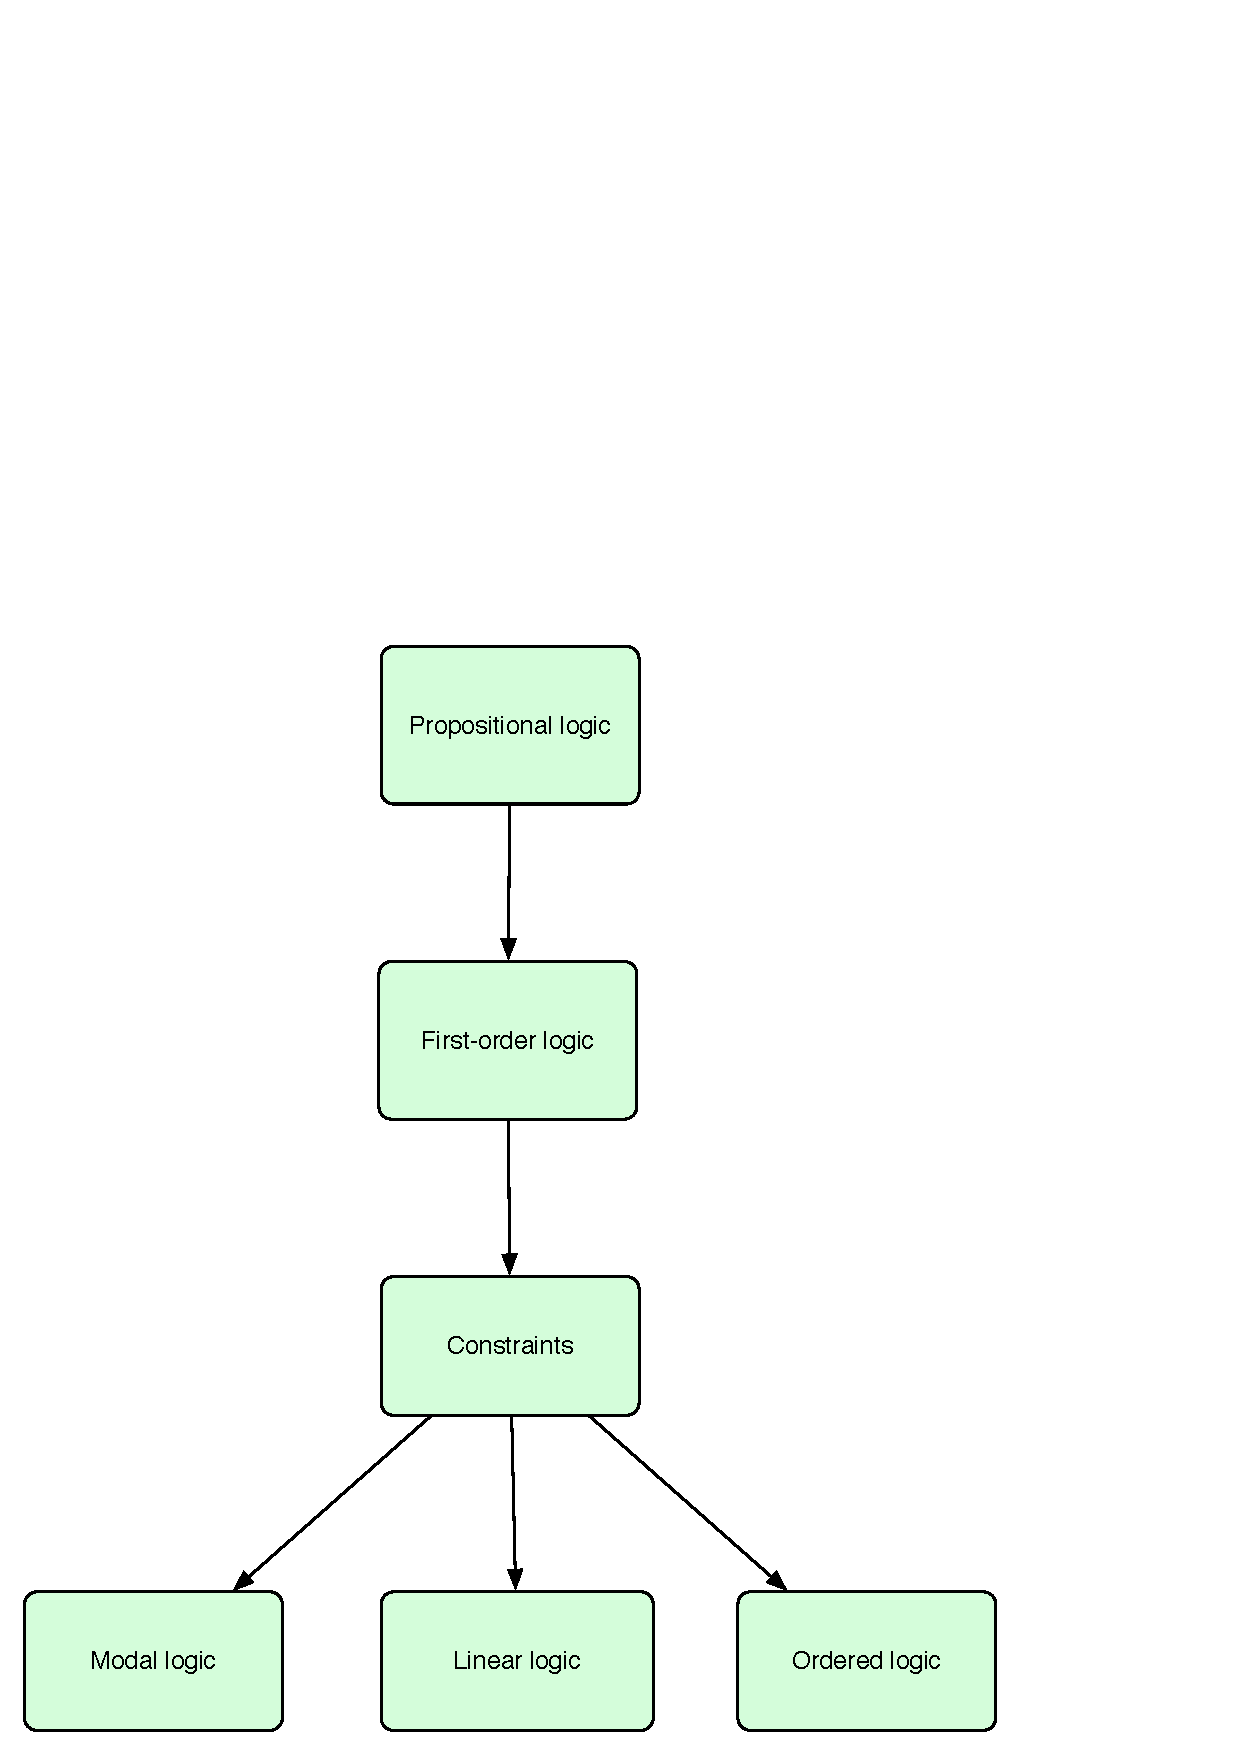
\includegraphics[scale=0.50]{graffle/logics.pdf}
  \end{center}
  \caption{Logics of this thesis}
  \label{graffle.logics}
\end{figure}
%%% Local Variables:
%%% mode: latex
%%% TeX-master: "../thesis"
%%% End:


\paragraph{Intuitionistic Propositional Logic.}
In Chapter~\ref{chapter.prop} we will review the inverse method.  Using
intuitionistic propositional logic as an example, we give a thorough description
of the polarized inverse method that will be used in the remainder of the
thesis.  We introduce focusing and polarities, give a polarized backward
calculus, and finally a polarized forward calculus in which we search for proofs
using the inverse method.  IPL is a good introduction to our methods because the
challenges exhibited by the other calculi are present there in their simplest
form.  Finally, we describe \emph{Imogen}, our implementation, and its
performance on established benchmark problems for IPL from the
ILTP~\cite{Raths.2007.JAR} library of intuitionistic propositional problems.
Imogen is among the best theorem provers for IPL.

\paragraph{Intuitionistic First-Order Logic.}
In Chapter~\ref{chapter.fol} we move to intuitionistic first order
logic.  There we enrich focusing and the
inverse method with first order quantification.  The important
operations of \emph{subsumption}, \emph{rule matching}, and
\emph{contraction} become significantly more difficult.  We extend the
results for propositional logic to this richer setting, and describe
the results of our implementation on the ILTP library of first-order
intuitionistic problems.  In short, Imogen has the best performance
of any existing intuitionistic theorem prover on first-order problems.

\paragraph{Intuitionistic Logic with Constraints.}
Chapter~\ref{chapter.constraints} describes an extension of the polarized inverse
method to first-order
intuitionistic logic with \emph{constraints}.  The motivation for constraints is
that as logics become more complex, the unification problem may not be instantly
solvable with a most general unifier.  It is beneficial to delay the solving of
unification equations until more information is available;  constraints provide
a way to delay computationally expensive choices.

\paragraph{Intuitionistic Modal Logic}
As the first application of constraints, in Chapter~\ref{chapter.modal}
we use the features developed in the previous chapter to design an efficient
theorem prover for some intuitionistic modal logics.  The constraints model
the visibility relation in the Kripke semantics.

\paragraph{Linear Logic}
A second application of constraints is to intuitionistic linear logic in
Chapter~\ref{chapter.linear}.  The constraints model linear resource management.
We compare this method of theorem proving against the only other theorem prover
for full first-order linear logic of which we are aware, Chaudhuri's
\emph{Linprover}.

\paragraph{Ordered Logic}
Finally, we use a different notion of constraints in Chapter~\ref{chapter.ordered}
where we implement a theorem prover for \emph{ordered logic}, a substructural
logic similar to linear logic without the exchange rule.  Ours is the only
existing implementation of a theorem prover for full ordered first-order
logic.

\section{Preliminaries}

\paragraph{Multisets.}

Let $\cU$ be a set of elements.  A \emph{(finite) multiset} $\Gamma$ of $\cU$
is a function $f$ from
$\cU$ to $\Nat$ where $f(x)=0$ for all but a finite number of elements of
$\cU$.  The empty multiset, written $\cdot$ is the function $\lambda\ x.\ 0$.
If $\Gamma=f$ is a multiset then $\Gamma, x = f'$
where $f'(x) = f(x)+1$ and $f'(y)=f(y)$ when $x\neq y$.
If $\Gamma'=f'$ then $\Gamma\Union\Gamma' = g$ where
$g(x) = f(x)+f'(x)$.  When we are writing both set and multiset union
in the same part of the text, we will use $X \uplus Y$ for multiset union.
For a multiset $\Gamma$, write $\dedup(\Gamma)$ for the set obtained by deleting
all duplicates in $\Gamma$.
The size of a set or multiset is written $\Card{\Gamma}$.

\paragraph{Ordered sequences.}

An \emph{ordered sequence} (or just \emph{sequence}) of (elements of a set) $X$ is either $[]$
or has the form $x:S$ where $x\in X$ and $S$ is an ordered sequence of X.
We abbreviate $x_1 : x_2 : \cdots : x_n : []$ as $[x_1,\ldots,x_n]$.

\paragraph{Notation.}

If $X$ is a set, let $\Set{X}$ be the powerset of $X$ and $\Aset{X}$ be
the set of ordered sequences of elements of $X$.  $\Aset{X}_n$ is the
set of sequences of $X$ with length $n$.

\paragraph{Forward and backward proof search.}
A proof procedure is called \emph{backward} (also \emph{top-down}) if it
proceeds by starting with a goal formula, decomposing that formula in some way
into subgoals, and searching for proofs of the subgoals.
Conversely, a proof-procedure is called \emph{forward} (also \emph{bottom-up})
if it begins with axioms, and uses the inference rules of the logic to infer new
formulas.  The terminology is admittedly confusing, but it is well established
and we adopt it in this thesis.  One way to avoid confusion is to think of a
proof as an inverted tree, whose root (the goal formula) is at the top and
leaves (the axioms) at the bottom\footnote{An analogy I also use is that of
jurisprudence in a kingdom.  A law may be proposed by the king, which is
decomposed into its various pieces to be enforced (top-down).  A law may also
emerge from the common people themselves, each of whom contribute a small part
to the final body of the law (bottom-up).}.
Resolution~\cite{Robinson.1965.JACM} and the inverse method are examples of forward
search.  Prolog's SLD resolution, tableaux~\cite{Hahnle.2001.Tableaux}
and matrix methods~\cite{Wallen.1990.Book} are examples of backward search.

\paragraph{Inference rules.}

\[
\infer={A}{A_1 & \ldots & A_n}
\]

\noindent
denotes multiple steps in a proof.

\paragraph{Assumed Background.}

We assume the reader is familiar with the basics of classical and
intuitionistic logic.  admissible inference rules, cut elimination
(non-)invertible rules

\section{XXX Notes}
\begin{itemize}
\item theorem provers with line counts to show what a pain writing
a theorem prover is.
\item show number of calls to automated prover in coq, HOL Light
\item differentiate producing proofs vs. verifying algorithm with reflection.
\end{itemize}

%%% Local Variables:
%%% mode: latex
%%% TeX-master: "thesis"
%%% End:
